% Fully-connected MLP schematic used on the title slide.
% Vector redraw of the standard "input / hidden layers / output" figure.
% Build:  pdflatex neural_network.tex
\documentclass[border=6pt]{standalone}
\usepackage{tikz}
\usepackage{amsmath}

\definecolor{inFill}{HTML}{C8E6C2}
\definecolor{inDraw}{HTML}{1B5E1B}
\definecolor{hidFill}{HTML}{C6C7EE}
\definecolor{hidDraw}{HTML}{1B1B6E}
\definecolor{outFill}{HTML}{F3CACA}
\definecolor{outDraw}{HTML}{7C1B1B}

\begin{document}
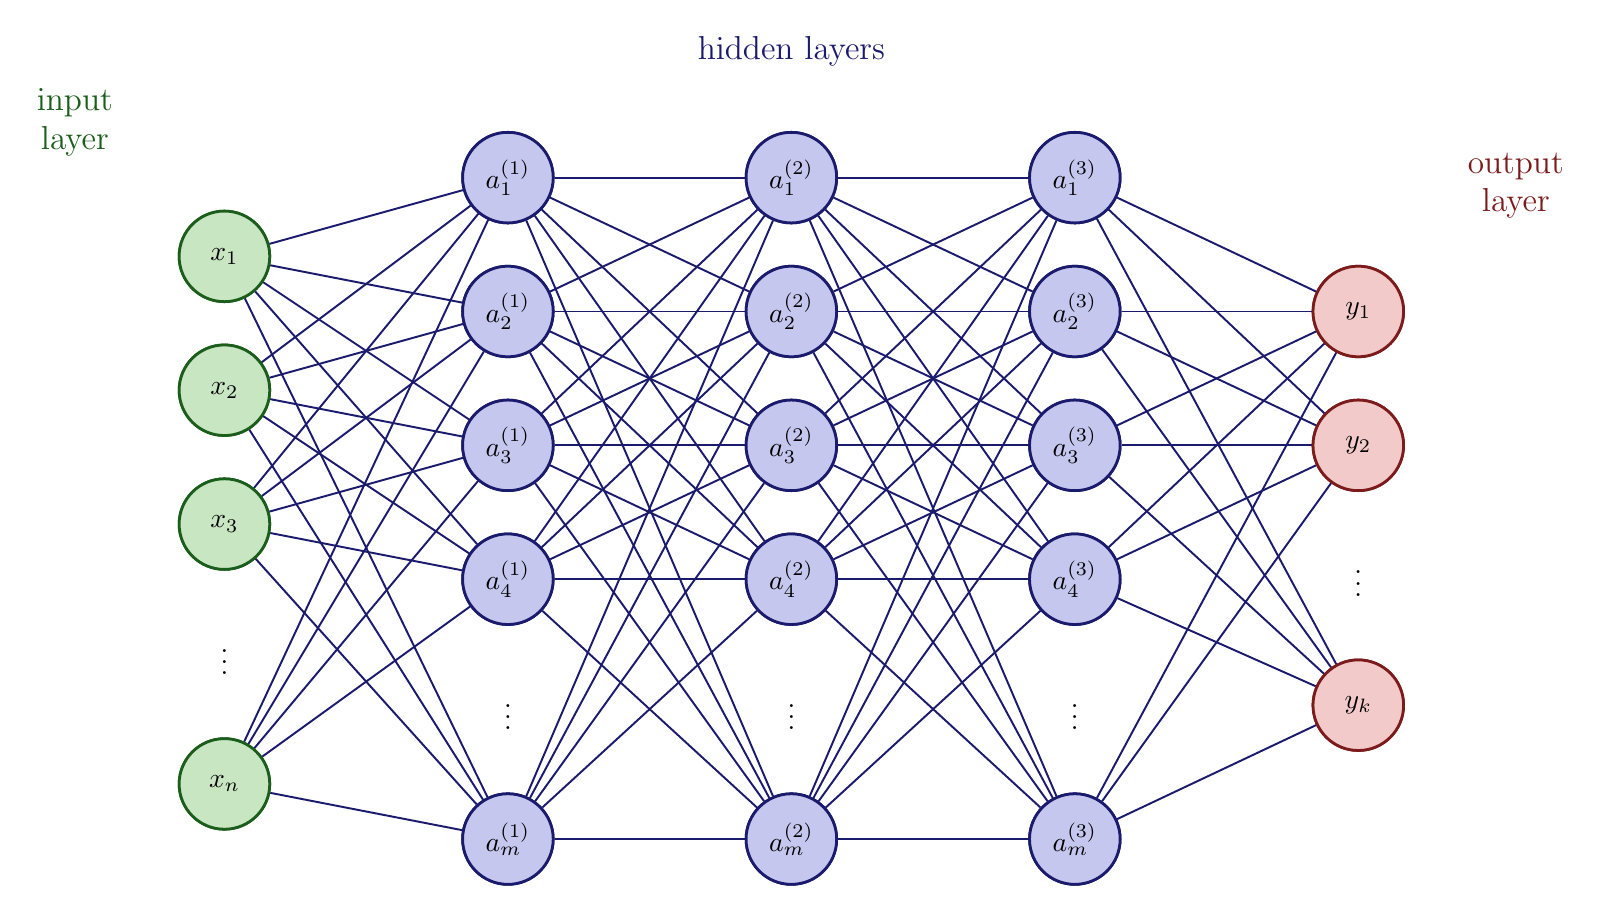
\begin{tikzpicture}[
  nd/.style={circle,draw,line width=1.0pt,minimum size=1.15cm,inner sep=0pt},
  inn/.style={nd,fill=inFill,draw=inDraw},
  hid/.style={nd,fill=hidFill,draw=hidDraw},
  outn/.style={nd,fill=outFill,draw=outDraw},
  ed/.style={draw=hidDraw,line width=0.7pt},
  lbl/.style={font=\large},
]

% ---- node columns -------------------------------------------------------
% input layer
\node[inn] (I1) at (0, 3.3)  {$x_1$};
\node[inn] (I2) at (0, 1.6)  {$x_2$};
\node[inn] (I3) at (0,-0.1)  {$x_3$};
\node       at (0,-1.75) {$\vdots$};
\node[inn] (I4) at (0,-3.4)  {$x_n$};

% three hidden layers
\foreach \L/\X in {1/3.6, 2/7.2, 3/10.8}{
  \node[hid] (H\L1) at (\X, 4.3)  {$a_1^{(\L)}$};
  \node[hid] (H\L2) at (\X, 2.6)  {$a_2^{(\L)}$};
  \node[hid] (H\L3) at (\X, 0.9)  {$a_3^{(\L)}$};
  \node[hid] (H\L4) at (\X,-0.8)  {$a_4^{(\L)}$};
  \node                at (\X,-2.45) {$\vdots$};
  \node[hid] (H\L5) at (\X,-4.1)  {$a_m^{(\L)}$};
}

% output layer
\node[outn] (O1) at (14.4, 2.6)  {$y_1$};
\node[outn] (O2) at (14.4, 0.9)  {$y_2$};
\node        at (14.4,-0.75) {$\vdots$};
\node[outn] (O3) at (14.4,-2.4)  {$y_k$};

% ---- fully-connected edges (nodes are redrawn on top afterwards) --------
\foreach \a in {I1,I2,I3,I4}
  \foreach \b in {H11,H12,H13,H14,H15}
    \draw[ed] (\a) -- (\b);
\foreach \a in {H11,H12,H13,H14,H15}
  \foreach \b in {H21,H22,H23,H24,H25}
    \draw[ed] (\a) -- (\b);
\foreach \a in {H21,H22,H23,H24,H25}
  \foreach \b in {H31,H32,H33,H34,H35}
    \draw[ed] (\a) -- (\b);
\foreach \a in {H31,H32,H33,H34,H35}
  \foreach \b in {O1,O2,O3}
    \draw[ed] (\a) -- (\b);

% redraw nodes on top of the edge mesh
\foreach \n/\t in {I1/{$x_1$},I2/{$x_2$},I3/{$x_3$},I4/{$x_n$}}
  \node[inn] at (\n) {\t};
\foreach \L in {1,2,3}{
  \foreach \i/\t in {1/1,2/2,3/3,4/4}
    \node[hid] at (H\L\i) {$a_\t^{(\L)}$};
  \node[hid] at (H\L5) {$a_m^{(\L)}$};
}
\foreach \n/\t in {O1/{$y_1$},O2/{$y_2$},O3/{$y_k$}}
  \node[outn] at (\n) {\t};

% ---- layer captions -----------------------------------------------------
\node[lbl,inDraw,align=center]  at (-1.9, 5.0) {input\\layer};
\node[lbl,hidDraw]              at ( 7.2, 5.9) {hidden layers};
\node[lbl,outDraw,align=center] at (16.4, 4.2) {output\\layer};

\end{tikzpicture}
\end{document}
